\section{Theoretical Framework}

\subsection{PDE Constrained Optimization}

\begin{frame}{PDE Constrained Optimization}
    \only<1>{
        \begin{block}{Motivation}
            Parameter dependence in PDEs:
            \begin{itemize}
                \item material properties
                \item velocities
                \item heat sources/sinks
                \item \dots
            \end{itemize}
        \end{block}
        \center{\textbf{How to determine optimal parameters?}}
    }

    \only<2>{
        \begin{block}{Problem Description, c.f.~\cite{Hinze2009}}
            We consider
            \begin{align*}
                &\min\limits_{\mu \in \mathcal{P}} \mathcal{J}(u, \mu) \qquad s.t.\\
                &e(u, \mu) = 0,
            \end{align*}
            where $e_\mu(u, v)$ encodes the PDE constraint
            \begin{equation*}
                e(u, \mu) := l_\mu(v) - a_\mu(u, v) \qquad \forall v \in V \text{ or } V_N
            \end{equation*}
        \end{block}
    }
\end{frame}

\begin{frame}{Notes on Differentiability}
    \only<1>{
        \begin{block}{Directional Derivative, c.f.~\cite{Hinze2009}}
            \vspace*{-8pt}
            \[ dF(x)[h] := \lim\limits_{t \rightarrow 0} \frac{F(x + th) - F(x)}{t} \in Y \]
        \end{block}
        
        \begin{block}{G\^{a}teaux Derivative, c.f.~\cite{Hinze2009}}
            \vspace*{-8pt}
            \[ dF(x) \in \mathcal{L}(X, Y) \]
        \end{block}

        \begin{block}{Fr\'{e}chet Derivative, c.f.~\cite{Hinze2009}}
            \vspace*{-8pt}
            \[ \norm[Y]{F(x + th) - F(x) - dF(x)[h]} = o(\norm[X]{h}), \norm[X]{h} \rightarrow 0 \]
        \end{block}
    }
        
    \only<2>{
        \begin{block}{Bilinear Form}
            Chain rule:
            \begin{align*}
                d_\mu a_\mu(u_\mu, v_\mu) \cdot \nu &= \partial_\mu a_\mu(u_\mu, v_\mu) \cdot \nu + \partial_u a_\mu(u_\mu, v_\mu)[d_\nu u_\mu] + \partial_v a_\mu(u_\mu, v_\mu)[d_\nu v_\mu] \\
                &= \partial_\mu a_\mu(u_\mu, v_\mu) \cdot \nu + a_\mu(d_\nu u_\mu, v_\mu) + a_\mu(u_\mu, d_\nu v_\mu)
            \end{align*}
            $d_\nu u_\mu, d_\nu v_\mu$ are also called \textbf{sensitivities}.
        \end{block}
    }
\end{frame}

\subsection{Trust-Region and BFGS Method}

\begin{frame}{Trust-Region Method}
    \begin{columns}
        \column{0.5\linewidth}
            \begin{figure}
                \centering
                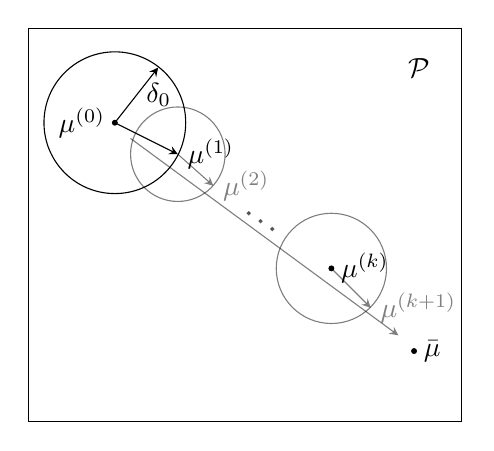
\begin{tikzpicture}[>=stealth]
                    \draw[fill=white] (-2.5,-2) rectangle (3,3);
                    \draw[black](2.2,2.5) node[right] (scrip) {$\mathcal{P}$};
                    \draw[fill=black] (-1.4,1.8) circle [radius=0.03, color=black];
                    \draw[black](-1.4,1.8) node[left] (scrip) {$\mu^{(0)}$};
                    \draw[fill=black] (2.4,-1.1) circle [radius=0.03, color=black];
                    \draw[black](2.4,-1.1) node[right] (scrip) {$\bar{\mu}$};
                    %\draw[->] (-1.2,1.6) -- (1.8,-0.9) node; %[midway,right] {Optimization};
                    \draw[->, opacity=0.5] (-1.2,1.6) -- (2.2,-0.9) node {}; %[midway,right] {Optimization};
                    \draw[->,black] (-1.4,1.8) -- (-0.85,2.5) node [midway,right] {$\delta_0$};
                    \draw[black] (-1.4,1.8) circle [radius=0.9, color=black];
                    \draw[->,black] (-1.4,1.8) -- (-0.6,1.4) node [right] {$\mu^{(1)}$};
                    \draw[black, opacity=0.5] (-0.6,1.4) circle [radius=0.6, color=black];
                    \draw[->,black, opacity=0.5] (-0.6,1.4) -- (-0.15,1) node [right] {$\mu^{(2)}$};
                    %\draw[fill=black, opacity=0.5] (0,0.85) circle [radius=0.03, color=black];
                    %\draw[fill=black, opacity=0.5] (0.15,0.75) circle [radius=0.03, color=black];
                    \draw[fill=black, opacity=0.5] (0.3,0.65) circle [radius=0.02, color=black];
                    \draw[fill=black, opacity=0.5] (0.45,0.55) circle [radius=0.02, color=black];
                    \draw[fill=black, opacity=0.5] (0.6,0.45) circle [radius=0.02, color=black];
                    \draw[fill=black] (1.35,-0.05) circle [radius=0.03, color=black];
                    \draw[black](1.35,-0.05) node[right] (scrip) {$\mu^{(k)}$};
                    \draw[black, opacity=0.5] (1.35,-0.05) circle [radius=0.7, color=black];
                    \draw[->,black, opacity=0.5] (1.35,-0.05) -- (1.85,-0.55) node [right] {$\mu^{(k+1)}$};
                \end{tikzpicture}
                \caption{Local adaptation (TR) on the domain,\\figure courtesy of Tim Keil}
            \end{figure}
        \column{0.5\linewidth}
            \begin{block}{Model function, c.f.~\cite{Kelley1999}}
                    \textbf{Idea:} Replace with simpler function $m^{(k)}$ modelling $\mathcal{J}$ around some point $x^{(k)}$.
            \end{block}
    \end{columns}
\end{frame}

\begin{frame}{Trust-Region Method}
    \begin{block}{Requirements, c.f.~\cite{Qian2017}}
        \begin{itemize}
            \item $\abs{\mathcal{J}(u_\mu, \mu) - \mathcal{J}_N(\mu)} \leq \Delta_{\mathcal{J}_N}(\mu)$, and
            \item $\mathcal{J}_N^{(k + 1)}(\mu^{(k + 1)}) \leq \mathcal{J}_N^{(k)}(\mu^{(k, 0)})$
        \end{itemize}
    \end{block}

    The second is equivalent to
    \begin{equation*}
        \mathcal{J}_N^{(k)}(\mu^{(k + 1)}) + \Delta_{\mathcal{J}_N^{(k)}}(\mu^{(k + 1)}) < \mathcal{J}_N^{(k)}(\mu^{(k)})
    \end{equation*}
\end{frame}

\begin{frame}{BFGS Method}
    \begin{block}{Newton Method, c.f.~\cite{Nocedal2006}}
        \vspace*{-8pt}
        \[ x^{(k + 1)} := x^{(k)} + \kappa^{(k)} d^{(k)}, \]
        \[ d^{(k)} := - {\mathcal{H}(x^{(k)})}^{-1} \nabla \mathcal{J}(x^{(k)}) \]
    \end{block}

    \only<2>{
        \begin{block}{Quasi Newton Method, c.f.~\cite{Kelley1999, Nocedal2006}}
            \vspace*{-8pt}
            \[  x^{(k + 1)} := x^{(k)} + \kappa^{(k)} d^{(k)}, \]
            \[ d^{(k)} := - {\mathcal{H}^{(k)}}^{-1} \nabla \mathcal{J}(x^{(k)}) \]
        \end{block}
    }
\end{frame}

\begin{frame}{BFGS Method}
    \begin{block}{BFGS Update Formula}
        \vspace*{-8pt}
        \[ \mathcal{H}^{(k + 1)} := \mathcal{H}^{(k)} + \frac{(y^{(k)} - \mathcal{H}^{(k)} s^{(k)}){(y^{(k)} - \mathcal{H}^{(k)} s^{(k)})}^T}{{(y^{(k)} - \mathcal{H}^{(k)} s^{(k)})}^T s^{(k)}}, \]
        \[ s^{(k)} := x^{(k + 1)} - x^{(k)}, \]
        \[ y^{(k + 1)} := \nabla \mathcal{J}(x^{(k + 1)}) - \nabla \mathcal{J}(x^{(k)}) \]
    \end{block}
\end{frame}